\documentclass{article}
\usepackage[margin=1in]{geometry}
\usepackage{amsmath, amssymb, amsthm}
\usepackage{enumitem}

% colored links
\usepackage{hyperref}
\hypersetup{
    colorlinks=true,
    linkcolor=blue,
    filecolor=magenta,      
    urlcolor=magenta,
    }

%Creating algorithms
\usepackage{algorithm}
\usepackage[noend]{algpseudocode}


% Inputting Python code
\usepackage[dvipsnames]{xcolor}
\definecolor{textblue}{rgb}{.2,.2,.7}
\definecolor{textred}{rgb}{0.54,0,0}
\definecolor{textgreen}{rgb}{0,0.43,0}
\usepackage{upquote}
\usepackage{listings}
\lstset{
    language=Python, 
    tabsize=4,
    basicstyle={\ttfamily},
    keywordstyle=\color{textblue},
    commentstyle=\color{textgreen},
    stringstyle=\color{textred},
    frame=none,
    columns=fullflexible,
    keepspaces=true,
    showstringspaces=false,
    xleftmargin=-15mm, % manual adjustment, figure out permanent solution
}

% Tcolorbox
\usepackage{tcolorbox}
\tcbuselibrary{skins,hooks}
\usetikzlibrary{shadows}

%Images
\usepackage{graphicx}
    \usepackage{subcaption}
    \usepackage{float}

%Creating Figures
\usepackage{tikz}
\usetikzlibrary{calc, math, matrix, graphs, positioning}
\usetikzlibrary{fit}
\usetikzlibrary{backgrounds}
\usetikzlibrary{hobby}

% the settings of tikz is used for the optimization of the graphs  
\usetikzlibrary{shapes, arrows, arrows.meta} % these are the parameters passed to the library to create the node graphs  
\tikzset{  
    auto,node distance =1.1 cm and 1.1 cm,% node distance is the distance between one node to other, where 1.5cm is the length of the edge between the nodes  
} 

%Formatting and Spacing
\setitemize[1]{noitemsep, parsep = 5pt, topsep = 5pt}
\setenumerate[1]{label = (\alph*), parsep = 1pt, topsep = 5pt}
\setlength\parindent{0pt}
\linespread{1.1}

% title
\title{\vspace{-1cm}CS 2051: Honors Discrete Mathematics \\Spring 2023 \texttt{generate\_schedule} Solution}
\author{Sarthak Mohanty }
\date{}

\begin{document}

\maketitle

The \lstinline{generate_schedule} function in this supplement seemed to pose quite the challenge! In this short document, we cover some initial approaches, the challenges/issues encountered, and finally the correct approach.

\subsection*{Initial Approach}

\vspace{3mm}
A common first implementation by many students was iteratively adding the minimal elements, as follows:

\begin{tcolorbox}[enhanced,title=Incorrect Approach,
    colframe=red!50!black,colback=red!10!white,
    arc=1mm,colbacktitle=red!10!white,
    fonttitle=\bfseries,coltitle=red!50!black,
    attach boxed title to top center=
    {yshift=-2mm,yshifttext=-1mm},
    boxed title style={
    interior style={fill=none,
    top color=red!30!white,
    bottom color=red!20!white}}]
    \begin{lstlisting}[belowskip=-10pt]
        def generate_schedule(elements: set, poset: set, num_processors: int) -> list[list]:
        
            scheduled_tasks = set()
            schedule = list()
         
            while(len(scheduled_tasks) != len(elements)):
                tasks = []
                
                # Look at all elements in the poset
                # and check if they are not in scheduled_tasks
                # and if they are not dependent on any elements in scheduled_tasks
                tasks = [v for v in elements if v not in scheduled_tasks\
                         and all(u in scheduled_tasks for u, _v in poset if _v == v)]
        
                # Take the first num_processors elements
                tasks = tasks[:num_processors]
        
                # Add the elements in tasks to scheduled_tasks
                scheduled_tasks = scheduled_tasks.union(tasks)
        
                schedule += [tasks]
            
            return schedule
    \end{lstlisting}
\end{tcolorbox}


This approach works fine for the example given in the docstrings, as shown below:

    \begin{lstlisting}[belowskip=-10pt]
        >>> generate_schedule({'1301', '1331', '1332', '4641', '2051', '3600', '3511'},
                {('1301', '1331'), ('1331', '1332'), ('1332', '4641'),\
                 ('2051', '3511'), ('1332', '3511'), ('1332', '3600')}, 2)
            [['1301', '2051'], ['1331'], ['1332'], ['4641', '3600'], ['3511']]
    \end{lstlisting}

    \begin{figure}[htbp]
        \captionsetup{width=.7\linewidth}
        \centering
        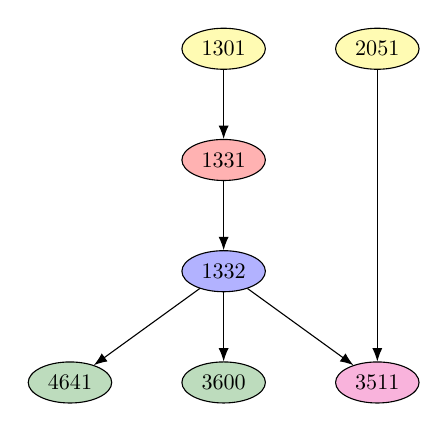
\begin{tikzpicture}[scale = 0.8, transform shape
        ,every node/.style ={ellipse, draw, minimum width = 0.9 cm},]  
            \node[fill=yellow!30] (1301) at (0,0) {1301};
            \node[fill=red!30] (1331) [below =of 1301] {1331};  
            \node[fill=blue!30] (1332) [below =of 1331] {1332};
            \node[fill=yellow!30] (2051) [right =of 1301] {2051};  
            \node[fill=ForestGreen!30] (3600) [below =of 1332] {3600};  
            \node[fill=ForestGreen!30] (4641) [left =of 3600] {4641};
            \node[fill=magenta!30] (3511) [right =of 3600] {3511};  
            \path[-Latex] (1301) edge (1331);
            \path[-Latex] (1331) edge (1332);
            \path[-Latex] (1332) edge (4641);
            \path[-Latex] (1332) edge (3600);
            \path[-Latex] (1332) edge (3511);
            \path[-Latex] (2051) edge (3511);
        \end{tikzpicture}
        \caption{Dependency graph of the sample poset, where the elements in row $i$ represents tasks that are ready to be scheduled at time $i$}
        \label{fig:sample_test_case}
    \end{figure}

\subsection*{The Issue}
    However, the above implementation does not always find the optimal schedule. Consider the following poset:

    \begin{lstlisting}[belowskip=-10pt]
        >>> generate_schedule({1, 2, 3, 4, 5}, {{(1, 5), (2, 5), (3, 4), (4, 5)}}, 2)
            [[1, 2], [3], [4], [5]]
    \end{lstlisting}

    In this case, the poset should schedule Task 3 first, but instead schedules Tasks 1 and 2 first, leading to an unoptimal schedule. 
    
    \vspace{2mm}
    Intuitively, this is because Task 3 has a further distance, or \textit{height} to the final Task $5$ in the dependency graph, so it should be scheduled first, as shown in Figure 
    \ref*{fig:correct_schedule}. However, our initial algorithm does not make this differentiation, and instead treats the poset as in Figure \ref*{fig:incorrect_schedule}.
\begin{figure}[htbp]
    \centering
    
    \begin{subfigure}[t]{.45\textwidth}
        \centering
        \captionsetup{width=.7\linewidth}
        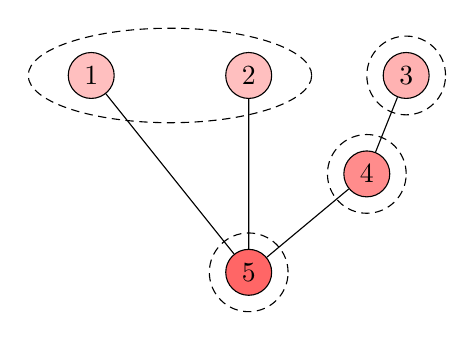
\begin{tikzpicture}
            [level distance=15mm,
            every node/.style={fill=red!60,circle,inner sep=3pt},
            level 1/.style={sibling distance=20mm,nodes={fill=red!45}},
            level 2/.style={sibling distance=10mm,nodes={fill=red!30}},
            level 3/.style={sibling distance=5mm,nodes={fill=red!25}}]
            ]
            \node(5) [draw] {5} [grow=up]
                child[level distance=12.5mm,sibling distance=15mm] {node(4) [draw] {4}
                    child[level distance=12.5mm] {node(3) [draw] {3} }
                    child[missing]
                }
                child[level distance=25mm] {node(2) [draw,fill=red!25] {2} }
                child[level distance=25mm] {node(1) [draw,fill=red!25] {1} };
            \draw[densely dashed] ($(1)!0.5!(2)$) circle [x radius=1.8cm, y radius=0.6cm];
            \draw[densely dashed] (3) circle[radius=0.5cm];
            \draw[densely dashed] (4) circle[radius=0.5cm];
            \draw[densely dashed] (5) circle[radius=0.5cm];
        \end{tikzpicture}
        \caption{Dependency graph demonstrating the initial approach.}
        \label{fig:incorrect_schedule}
    \end{subfigure}
    \begin{subfigure}[t]{.45\textwidth}
        \centering
        \captionsetup{width=.7\linewidth}
        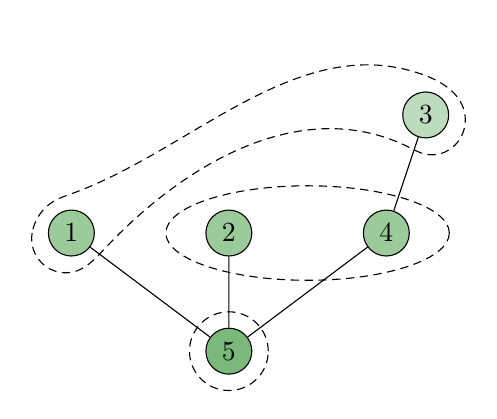
\begin{tikzpicture}
            [level distance=15mm,
            every node/.style={fill=ForestGreen!60,circle,inner sep=3pt},
            level 1/.style={sibling distance=20mm,nodes={fill=ForestGreen!45}},
            level 2/.style={sibling distance=10mm,nodes={fill=ForestGreen!30}},
            level 3/.style={sibling distance=5mm,nodes={fill=ForestGreen!25}}]
            \node(5) [draw] {5} [grow=up]
                child {node(4) [draw] {4}
                    child {node(3) [draw] {3} }
                    child[missing]
                }
                child {node(2) [draw] {2} }
                child {node(1) [draw] {1} };
            \draw[densely dashed, use Hobby shortcut] 
                ([xshift=-.2cm]1.west) .. ([yshift=-.2cm]1.south).. ([xshift=.2cm]1.south east)..([yshift=-.2cm]3.south west)..([yshift=-.2cm]3.south).. ([xshift=.2cm]3.east)..([yshift=.2cm]3.north) .. ([yshift=.2cm] 1.north) .. ([yshift=.2cm] 1.north west) .. ([xshift=-.2cm]1.west);
            \draw[densely dashed] (5) circle[radius=0.5cm];
            \draw[densely dashed] ($(2)!0.5!(4)$) circle [x radius=1.8cm, y radius=0.6cm];
        \end{tikzpicture}
        \caption{Dependency graph where elements are ordered by height.}
        \label{fig:correct_schedule}
    \end{subfigure}
    \caption{Two schedules, each illustrating a different approach to the problem.}
    \label{fig:edge_case}
\end{figure}


\subsection*{Revised Approach}
    After understanding why our initial algorithm fails, it is easy to see how to correct it.
    \begin{enumerate}[label = \arabic*.]
        \item Before scheduling any tasks, we should calculate the height of every element by finding the maximum distance to any \textit{maximal} elements (elements which do not have any dependents).
        \item After obtaining tasks which are ready to be scheduled, we should ``rank" them based on their calculated heights in the dependency graph.
    \end{enumerate}
    The updated approach is shown below:
    \begin{tcolorbox}[enhanced,title=Correct Approach,
        colframe=green!50!black,colback=green!10!white,
        arc=1mm,colbacktitle=green!10!white,
        fonttitle=\bfseries,coltitle=green!50!black,
        attach boxed title to top center=
        {yshift=-2mm,yshifttext=-1mm},
        boxed title style={
        interior style={fill=none,
        top color=green!30!white,
        bottom color=green!20!white}}]
        \begin{lstlisting}[belowskip=-10pt]
        def generate_schedule(elements: set, poset: set, num_processors: int) -> list[list]:
        
            scheduled_tasks = set()
            schedule = list()

            # Compute the height of each element
            heights = { x: 0 for x in elements }
            for x in topological_sort(elements, poset)[::-1]:
                dependents = [ v for _u, v in poset if _u == x ]
                if dependents:
                    # height of x is 1 + max height of children
                    heights[x] = 1 + max(heights[y] for y in dependents)
         
            while(len(scheduled_tasks) != len(elements)):
                tasks = []
                
                # Look at all elements in the poset
                # and check if they are not in scheduled_tasks
                # and if they are not dependent on any elements in scheduled_tasks
                tasks = [v for v in elements if v not in scheduled_tasks\
                         and all(u in scheduled_tasks for u, _v in poset if _v == v)]

                # Sort the elements by their depth in the poset
                tasks = sorted(tasks, key=lambda x: heights[x], reverse=True)
        
                # Take the first num_processors elements
                tasks = tasks[:num_processors]
        
                # Add the elements in tasks to scheduled_tasks
                scheduled_tasks = scheduled_tasks.union(tasks)
        
                schedule += [tasks]
            
            return schedule
        \end{lstlisting}
\end{tcolorbox}

\begin{lstlisting}
        >>> generate_schedule({1, 2, 3, 4, 5}, {{(1, 5), (2, 5), (3, 4), (4, 5)}}, 2)
            [[1, 3], [2, 4], [5]]
\end{lstlisting}

\subsection*{Time Complexity}
    The current implementation of this algorithm yields a time complexity of $\mathcal{O}(n^{3})$, where $n$ is the number of elements in the poset. This is because we sort each of the elements (taking time $\mathcal{O}(n\log(\text{n}))$) as well as compute each of the minimal elements (taking time $\mathcal{O}(n^{2})$) time at \textit{each} iteration.

    \vspace{2mm}
    However, by using more efficient representations for our data, as well as external data structures such as priority queues, we can reduce the time complexity considerably. \underline{We will not reveal the optimal time complexity here}, for reasons that will be clear in the end of the semester.

\end{document}